\documentclass[handout, font=12pt]{ximera}

\title{Fractions: Graphing}   % Use xmlatex all -s to compile when SERVE refuses to work.
\author{Kelly Stady}
\license{CC: 0}         % replace with an appropriate license, or set it in xmPreamble

\begin{document}   

\begin{abstract}

\end{abstract}

\maketitle

\label{xim:FractionsGraph}


\section*{Graphing Fractions on a Number Line}

To graph a \textbf{proper fraction}, divide the distance from 0 to 1 into $n$ equal parts, where $n$ is the denominator of the fraction.  Then start at 0 and use the numerator to determine the number of places to move to the right.

\begin{example}

Graph the \textbf{proper fraction} $\textstyle \frac{3}{4}.$ 

\begin{explanation}
  
Since the denominator is $4,$ divide the distance from $0$ to $1$ into $4$ equal parts.  Then start at $0$ and move $3$ parts to 
the right, since the numerator is $3.$

\begin{center}
\begin{tikzpicture}[>=stealth]
        % Draw number line and mark 0, 1, 3/4
        \draw[thick, <->] (0,0)--(6,0) node at (1,-0.3)  {0} node at (5, -0.3) {1} node at (4,0.6) {$\displaystyle \frac{3}{4}$};

        %Tickmarks
        \draw[thick] (1,-0.1)--(1, 0.1);
        \draw[thick] (2,-0.1)--(2, 0.1);
        \draw[thick] (3,-0.1)--(3, 0.1);
        \draw[thick] (4,-0.1)--(4, 0.1);
        \draw[thick] (5,-0.1)--(5, 0.1);

        % 3/4 point
        \fill (4,0) circle (2pt);
\end{tikzpicture}

% Alt Text
\xmalt{A horizontal number line showing the interval from 0 to 1, divided into four equal segments. 
The integer 0 is labeled at the first tick mark, and the integer 1 is labeled at the fifth tick mark. A solid black dot is placed 
on the third tick mark from 0 and labeled as three-fourths.}
\end{center}

\end{explanation}
\end{example}

To graph \textbf{improper fractions}, we continue the process and divide the distances between each whole number into $n$ equal parts.

\begin{example}

Graph the \textbf{improper fraction} $\textstyle \frac{7}{4}.$ 

\begin{explanation}

Since the denominator is $4,$ divide the distance between each whole number into $4$ equal parts.  Then start at $0$ and count $7$ 
parts to the right, since the numerator is $7.$

\begin{center}
\begin{tikzpicture}[>=stealth]
        % Draw longer number line and mark 0, 1, 2, and fractions
        \draw[thick, <->] (0,0)--(10,0);

        % Labels below the line
        \node at (1,-0.3) {0};
        \node at (5,-0.3) {1};
        \node at (9,-0.3) {2};
        \node at (8,0.6) {$\displaystyle \frac{7}{4}$};

        % Tickmarks (0 to 2 in quarters)
        % 0 at 1, 1 at 5, 2 at 9. Spacing is 1 unit per 1/4.
        \foreach \x in {1,2,3,4,5,6,7,8,9}
          \draw[thick] (\x,-0.1)--(\x, 0.1);

        % Point
        \fill (8,0) circle (2pt); % 7/4 point
\end{tikzpicture}

% alt text 
\xmalt{A horizontal number line extending from 0 to 2, divided into eight equal segments. The integers 0, 1, and 2 are 
labeled. A single solid black dot is placed at the seventh tick mark from 0 and labeled as seven-fourths.}
\end{center}

\begin{remark}
Notice that $\frac{7}{4}$ is equivalent to $1 \frac{3}{4}$ since it lies $\frac{3}{4}$ of the way between 1 and 2.
\end{remark}

\end{explanation}
\end{example}

To graph a \textbf{mixed number}, first locate the whole number part on the number line. Next, divide the distance between 
that whole number and the next whole number into $n$ equal parts, where $n$ is the number in the denominator.  Then start 
at the whole number part and graph the fractional part.

\begin{example}

Graph the \textbf{mixed number} $\textstyle 2 \frac{1}{5}.$ 

\begin{explanation}

Since the denominator is $5,$ divide the distance between the whole numbers $2$ and $3$ into $5$ equal parts.  Then start at $2$ and 
move $1$ part to the right, since the numerator is $1.$

\begin{center}
\begin{tikzpicture}[thick, >=stealth]
  % 1. Draw the number line from -0.5 to 3.5
  \draw[<->] (-0.5,0) -- (9.5,0);

  % 2. Major Tickmarks for whole numbers 0, 1, 2, 3
  % Placed at x=0, x=3, x=6, x=9 for clear spacing
  \foreach \x/\label in {0/0, 3/1, 6/2, 9/3} {
    \draw (\x, 0.15) -- (\x, -0.15) node[below] {\label};
  }

  % 3. Minor Tickmarks between 2 and 3 (5 equal parts)
  % The distance between 6 and 9 is 3 units. 3 / 5 = 0.6 spacing.
  \foreach \i in {1,2,3,4} {
    \draw (6 + 0.6*\i, 0.1) -- (6 + 0.6*\i, -0.1);
  }

  % 4. Graph the point 2 1/5 (the first tick after 2)
  \fill (6.6, 0) circle (2.5pt);

  % Optional: Label the point itself
  \node at (6.6, 0.6) {$\displaystyle 2\frac{1}{5}$};
\end{tikzpicture}

% Alt Text
\xmalt{A horizontal number line labeled with the whole numbers 0, 1, 2, and 3. The segment between 2 and 3 is divided into five equal parts. A 
solid black dot is placed on the first tick mark after 2 and labeled as the mixed number two and one-fifth.}
\end{center}

\end{explanation}
\end{example}

\begin{remark}
Negative fractions can be graphed in a similar manner.
\end{remark}


\begin{problem}  
  Identify the position of the letter $A$ on the number line.


\begin{center}   
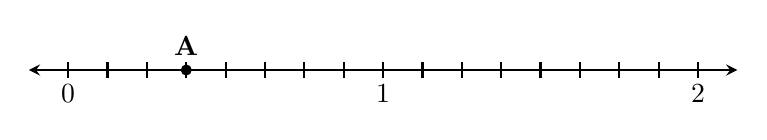
\begin{tikzpicture}[>=stealth]
        \draw[thick, <->] (0.5,0)--(9.5,0) node at (1,-0.3) {0} node at (5, -0.3) {1} node at (9, -0.3) {2} node at (2.5, 0.3) {\textbf{A}};
        %node at (8.5, 0.3) {\textbf{B}};
        \draw[thick] (1,-0.1)--(1, 0.1);
        \draw[thick] (1.5,-0.1)--(1.5, 0.1);
        \draw[thick] (2,-0.1)--(2, 0.1);
        \draw[thick] (2.5,-0.1)--(2.5, 0.1);
        \draw[thick] (3,-0.1)--(3, 0.1);
        \draw[thick] (3.5,-0.1)--(3.5, 0.1);
        \draw[thick] (4,-0.1)--(4, 0.1);
        \draw[thick] (4.5,-0.1)--(4.5, 0.1);
        \draw[thick] (5,-0.1)--(5, 0.1);
        \draw[thick] (5.5,-0.1)--(5.5, 0.1);

        \draw[thick] (6,-0.1)--(6, 0.1);
        \draw[thick] (6.5,-0.1)--(6.5, 0.1);
        \draw[thick] (7,-0.1)--(7, 0.1);
        \draw[thick] (7.5,-0.1)--(7.5, 0.1);
        \draw[thick] (8,-0.1)--(8, 0.1);
        \draw[thick] (8.5,-0.1)--(8.5, 0.1);
        \draw[thick] (9,-0.1)--(9, 0.1);
        \fill (2.5,0) circle (2pt);
        %\fill (8.5,0) circle (2pt);
\end{tikzpicture}

\xmalt{A horizontal number line extending from 0 to 2. The distance between each whole number is divided into eight equal parts. 
 Point A is marked with a solid black dot and is located at the third tick mark after 0.}
 
\end{center}

$A =\frac{\answer{3}}{\answer{8}} $


\begin{hint}
To find the denominator of $A,$ identify the number of spaces between each whole number.  To find the numerator, start
at 0 and count the number of tick marks to get to $A.$
\end{hint}


 
\end{problem}


\begin{problem}
Identify the position of the letter $B$ on the number line.

~ \\[3em]

\begin{center}
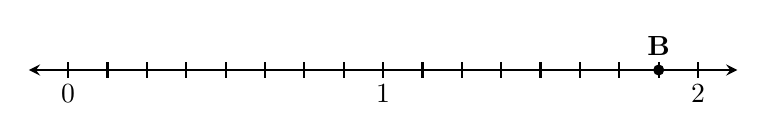
\begin{tikzpicture}[>=stealth]
        \draw[thick, <->] (0.5,0)--(9.5,0) node at (1,-0.3)  {0} node at (5, -0.3) {1} node at (9, -0.3) {2} node at (8.5, 0.3) {\textbf{B}};
        
        \draw[thick] (1,-0.1)--(1, 0.1);
        \draw[thick] (1.5,-0.1)--(1.5, 0.1);
        \draw[thick] (2,-0.1)--(2, 0.1);
        \draw[thick] (2.5,-0.1)--(2.5, 0.1);
        \draw[thick] (3,-0.1)--(3, 0.1);
        \draw[thick] (3.5,-0.1)--(3.5, 0.1);
        \draw[thick] (4,-0.1)--(4, 0.1);
        \draw[thick] (4.5,-0.1)--(4.5, 0.1);
        \draw[thick] (5,-0.1)--(5, 0.1);
        \draw[thick] (5.5,-0.1)--(5.5, 0.1);

        \draw[thick] (6,-0.1)--(6, 0.1);
        \draw[thick] (6.5,-0.1)--(6.5, 0.1);
        \draw[thick] (7,-0.1)--(7, 0.1);
        \draw[thick] (7.5,-0.1)--(7.5, 0.1);
        \draw[thick] (8,-0.1)--(8, 0.1);
        \draw[thick] (8.5,-0.1)--(8.5, 0.1);
        \draw[thick] (9,-0.1)--(9, 0.1);
        %\fill (2.5,0) circle (2pt);
        \fill (8.5,0) circle (2pt);
\end{tikzpicture}

% Alt Text
 \xmalt{A horizontal number line extending from 0 to 2.  The whole numbers 0, 1 and 2 are labeled.  The distance between each whole 
 number is divided into eight equal parts.  Point B is located at the fifteenth tick mark after 0 or equivalently at the seventh tick mark after 1.}
 
\end{center}


\begin{hint}
To find the denominator of $B,$ identify the number of spaces between each whole number.  To find the numerator, start
at 0 and count the number of tickmarks to get to $B.$  Equivalently, start at 1 and count the number
of tickmarks to get to $B,$ then write the result as a mixed number.
\end{hint}


\begin{selectAll}
\choice[correct]{$\displaystyle 1 \frac{7}{8}$}
\choice{$\displaystyle \frac{16}{8}$}
\choice[correct]{$\displaystyle  \frac{15}{8}$}
\choice{$\displaystyle  1 \frac{5}{8}$}
\choice{$\displaystyle  \frac{5}{8}$}
\choice{$\displaystyle  \frac{7}{8}$}
\end{selectAll}

\end{problem}

\begin{problem}
Identify the position of the letter $C$ on the number line.

\begin{center}
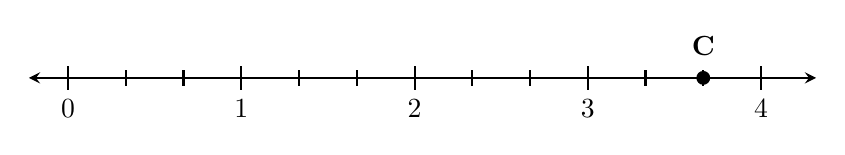
\begin{tikzpicture}[thick, >=stealth]
  % 1. Draw the number line from 0 to 4.5
  \draw[<->] (-0.5,0) -- (9.5,0);


  % 3. Major Tickmarks for whole numbers 1, 2, 3, 4
  % Placed at intervals of 2.2 unit for clean spacing (Total 8.8 for x=4)
  \foreach \x/\label in {0/0, 2.2/1, 4.4/2, 6.6/3, 8.8/4} {
    \draw (\x, 0.15) -- (\x, -0.15) node[below] {\label};
  }

  % 4. Minor Tickmarks between each whole number (3 equal parts)
  % Interval is 2.2 / 3 = 0.733
  \foreach \w in {0, 2.2, 4.4, 6.6} {
    \foreach \i in {1,2} {
      \draw ({\w + 0.733*\i}, 0.1) -- ({\w + 0.733*\i}, -0.1);
    }
  }

  % 5. Graph Point C at 3 2/3 (second tick after 3)
  % 6.6 + (2 * 0.733) = 8.066
  \fill (8.066, 0) circle (2.5pt);
  \node at (8.066, 0.4) {\textbf{C}};

\end{tikzpicture}
% alt text
\xmalt{A horizontal number line extending from 0 to 4. The whole numbers 0, 1, 2, 3 and 4 are labeled.  The distance between each whole number
has been divided into three equal parts.  Point C is labeled with a solid black dot and is located at the second tick mark after 3.}
\end{center}


\begin{selectAll}
\choice{$\displaystyle 3\frac{1}{2}$}
\choice{$\displaystyle  3 \frac{3}{4}$}
\choice{$\displaystyle  \frac{2}{3}$}
\choice{$\displaystyle  \frac{11}{2}$}
\choice[correct]{$\displaystyle  3 \frac{2}{3}$}
\choice[correct]{$\displaystyle  \frac{11}{3}$}
\end{selectAll}

\end{problem}

\end{document}